% THIS IS SIGPROC-SP.TEX - VERSION 3.1
% WORKS WITH V3.2SP OF ACM_PROC_ARTICLE-SP.CLS
% APRIL 2009
%
% It is an example file showing how to use the 'acm_proc_article-sp.cls' V3.2SP
% LaTeX2e document class file for Conference Proceedings submissions.
% ----------------------------------------------------------------------------------------------------------------
% This .tex file (and associated .cls V3.2SP) *DOES NOT* produce:
%       1) The Permission Statement
%       2) The Conference (location) Info information
%       3) The Copyright Line with ACM data
%       4) Page numbering
% ---------------------------------------------------------------------------------------------------------------
% It is an example which *does* use the .bib file (from which the .bbl file
% is produced).
% REMEMBER HOWEVER: After having produced the .bbl file,
% and prior to final submission,
% you need to 'insert'  your .bbl file into your source .tex file so as to provide
% ONE 'self-contained' source file.
%
% Questions regarding SIGS should be sent to
% Adrienne Griscti ---> griscti@acm.org
%
% Questions/suggestions regarding the guidelines, .tex and .cls files, etc. to
% Gerald Murray ---> murray@hq.acm.org
%
% For tracking purposes - this is V3.1SP - APRIL 2009

%\documentclass{acm_proc_article-sp}
\documentclass{sig-alternate}

\usepackage{soul,color}
\usepackage{url}
\usepackage{booktabs}
\usepackage{multirow}
\usepackage{enumitem}

\usepackage{blindtext, graphicx}
\usepackage{color}
\usepackage{amsmath}
\usepackage{url}

\newcommand{\fixme}[1]{}
\newcommand{\note}[1]{\fcolorbox{red}{yellow}{\textbf{\begin{minipage}{0.4\textwidth}#1\end{minipage}}}}


\usepackage[acronym]{glossaries}
%Term definitions
% Example of usage: \gls{IoT}

%to remove copyright that seems to not be required
\makeatletter
\def\@copyrightspace{\relax}
\makeatother

\begin{document}

\title{Towards a patch and bug analyser based on GitHub APIs  \titlenote{
CS474, December 9th, 2016, Chicago, USA. 
Copyright retained by the authors.}}


%
% You need the command \numberofauthors to handle the 'placement
% and alignment' of the authors beneath the title.
%
% For aesthetic reasons, we recommend 'three authors at a time'
% i.e. three 'name/affiliation blocks' be placed beneath the title.
%
% NOTE: You are NOT restricted in how many 'rows' of
% "name/affiliations" may appear. We just ask that you restrict
% the number of 'columns' to three.
%
% Because of the available 'opening page real-estate'
% we ask you to refrain from putting more than six authors
% (two rows with three columns) beneath the article title.
% More than six makes the first-page appear very cluttered indeed.
%
% Use the \alignauthor commands to handle the names
% and affiliations for an 'aesthetic maximum' of six authors.
% Add names, affiliations, addresses for
% the seventh etc. author(s) as the argument for the
% \additionalauthors command.
% These 'additional authors' will be output/set for you
% without further effort on your part as the last section in
% the body of your article BEFORE References or any Appendices.

\numberofauthors{3} %  in this sample file, there are a *total*
% of EIGHT authors. SIX appear on the 'first-page' (for formatting
% reasons) and the remaining two appear in the \additionalauthors section.
%
\author{
% You can go ahead and credit any number of authors here,
% e.g. one 'row of three' or two rows (consisting of one row of three
% and a second row of one, two or three).
%
% The command \alignauthor (no curly braces needed) should
% precede each author name, affiliation/snail-mail address and
% e-mail address. Additionally, tag each line of
% affiliation/address with \affaddr, and tag the
% e-mail address with \email.
%
% 1st. author
\alignauthor
Marco Arnaboldi \\
        \affaddr{University of Illinois at Chicago}\\
%        \affaddr{Milano, Italy}\\
       \email{\small{marnab2@uic.edu}}
% 2nd. author
\alignauthor
Alessandro Pappalardo \\
        \affaddr{University of Illinois at Chicago}\\
%        \affaddr{Milano, Italy}\\
        \email{\small{add mail}}
% 3rd. author
\alignauthor 
Andrea Tirinzoni \\
        \affaddr{University of Illinois at Chicago}\\
%        \affaddr{Milano, Italy}\\
        \email{\small{add mail}}
}


% There's nothing stopping you putting the seventh, eighth, etc.
% author on the opening page (as the 'third row') but we ask,
% for aesthetic reasons that you place these 'additional authors'
% in the \additional authors block, viz.
% Just remember to make sure that the TOTAL number of authors
% is the number that will appear on the first page PLUS the
% number that will appear in the \additionalauthors section.

\maketitle

\begin{abstract}

\end{abstract}

% A category with the (minimum) three required fields
%\category{H.4}{none}{}

% Suggestions for the keyword: Embedded operating systems, middleware, runtime support, resource management, and virtual machines

\sloppy


\section{Introduction}
\label{sec:introduction}

\section{System design and implementation}
\label{sec:implementation}

\begin{figure}
  \centering
  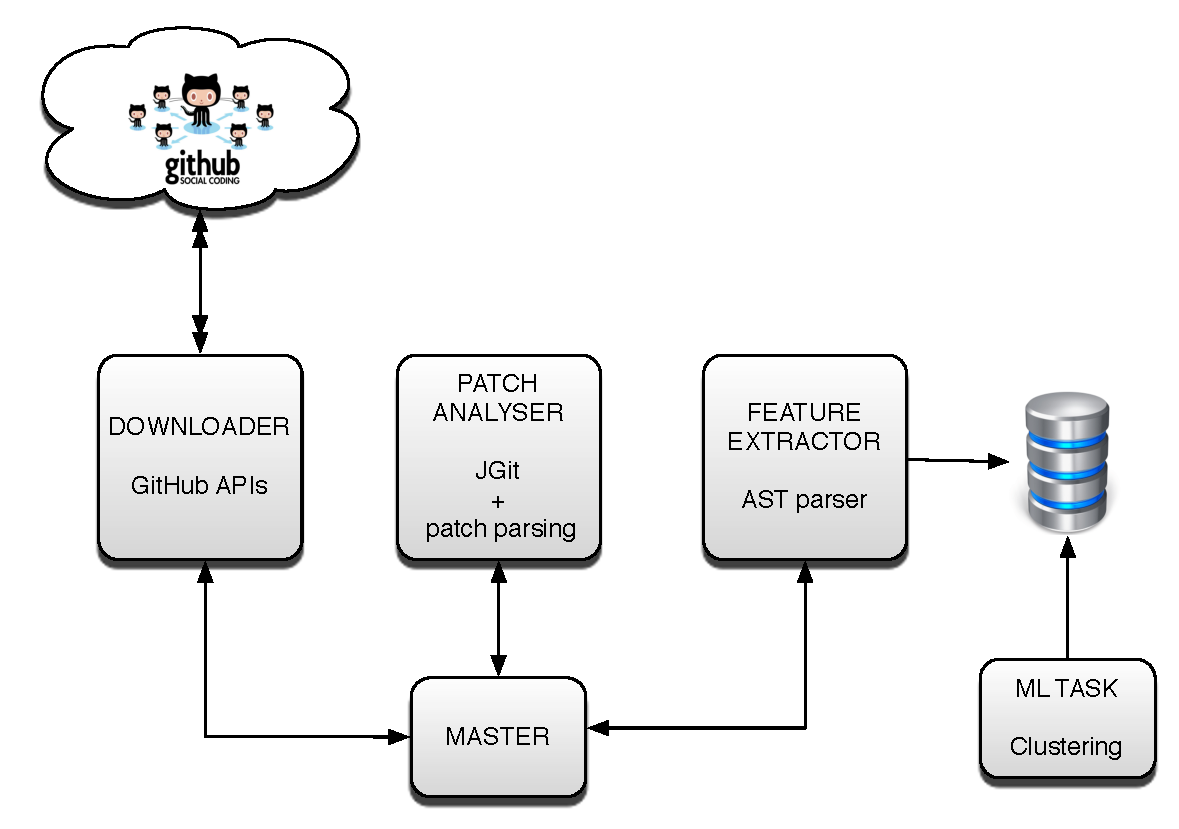
\includegraphics[width=0.5\textwidth]{pictures/overallArch.pdf}
  \caption{Overview of the proposed approach}
  \label{fig:overall}
\end{figure}


The system was thought taking into account two main features: scalability and high patch-analysed ratio. In order to achieve these two goals the system was designed as what we define: a replicable and single stage scalable pipeline. The main idea, as shown in Figure \ref{fig:overall}, is to have a pipeline of stages that are in charge to download repositories and issues related to them, then to extract patches from those and then mix the just retrieved data in order to extract features for the machine leaning task. In order to improve the scalability, the development and future extension every stage was developed independently from the others. In this direction we adopted reactive programming paradigm using the Akka framework, defining each stage as an actor. Those actors are of three kinds, one for each stage of the pipeline: the downloader, the patch-analyser and the feature-extractor. Actually there is a fourth actor -the master- in charge to manage the communication flow between the others and to instantiate new actors if needed. The pipeline is meant to be replicable in the sense that instantiating more than one stage at time it's possible to have several pipelines working in parallel. The mean of single stage scalable lies in the fact that it is also possible to set the number of replicas of a single stage independently by the other two. This means that in case a stage is slower than the others, just replicate its functionalities with one more actor of the same kind and in this way the bottleneck will be less strict. All of these parameters can be fixed inside a configuration class, which contains parameters for a full customization of the system. The output of the pipeline is a dataset representing a set of features describing the changes made in order to fix an issue in the repository. These data are then used to feed the machine learning task, that tries to find common pattern between changes and try to cluster them together. In this section we are going to go deep into each pipeline's stage and its duties. 
\subsection{Downloader}
This stage of the pipeline is in charge to directly manage the GitHub APIs. These are REST APIs based on the weel known JSON format. In detail the system exploits REST call with OAuth authorization in order to increase the number of request per hour allowed (5000). The first request the downloader makes is for retrieving a list of issues that were closed. Once those are retrieved via parsing the JSON response they are filtered, all meaningless ones are discarded, where meaningless means those issues related to repositories not public or where the coommit that closed those issues is missing. In order to retrieve the information necessary to the filter step different API calls are made and the responses are mixed together in order to extract the necessary parameters for the filter. Once the repo is marked as good the downloader downloads it and send information to local repository path, relative issue and closing commit to the patch analyser stage. 
\subsection{Patch Analyser}
This stage of the pipeline is in charge of extracting the modifications introduced by a commit, given a commit hash from the previous stage. We take advantage of the JGit library to extract the location of the modifications performed by the commit in the source code.
\subsection{Feature Extractor}
This stage of the pipeline receives information about diffs in a patch file and extracts features from the involved source files. The goal is to obtain a numerical dataset where each sample represents a single diff in a patch file. First, the files before and after the change are parsed to generate their AST. Then, the AST is used to extract features from the portion of code that has changed. We define a feature as the number of occurrences of some semantic attribute in the code (e.g., a for loop, a certain operation, a lambda expression, and so on). A sample is then the vector of features in the code before and after the change. Thus, we obtain a (very sparse) numerical dataset onto which we can apply clustering techniques. 
\subsection{Machine Learning} 
We apply clustering on the numerical dataset generated by our system. We decided to consider only hierarchical clustering since it provides the most general results (we get a cluster dendogram that we can cut in the desired number of clusters). We adopt the cosine similarity measure since it is the most suitable for our kind of dataset (high-dimensional and sparse feature vectors). We implement our clustering script in R, so that it can be easily integrated with Spark in case we need to scale to larger datasets.
\section{Experimental Results}
\label{sec:results}


\section{Limitations}
\label{sec:limitations}

Our current approach has several limitations. First, we are considering only Java projects. However, our code is easily extensible to support other languages. Second, we can generated only small datasets due to the restrictions imposed by GitHub on API calls. Our current solution is to run the system multiple times, waiting the necessary time between runs, to collect more samples. Our main limitation is that we are not able to exploit bug reports as we were expecting. The majority of bug reports on GitHub are poorly written and the application of some text mining algorithm on them would lead to very bad results. Thus, at the moment we lack a method to evaluate our clusters in a meaningful way. Our last limitation is that we are considering only a simple feature set. However, our code can be easily extended to include much more complicated features, even those representing dependencies between code constructs.
\section{Conclusion and future work}
\label{sec:conclusion}

We presented a new approach to analyze git patches and bugs based on Machine Learning techniques. We demonstrated how we can obtain some meaningful results even by implementing a simple system with several limitations. We mentioned that our system can be easily extended to obtain much more interesting results. As a future work, we intend to improve our system's capabilities to see whether we are, indeed, able to detect more useful patterns.


%
% The following two commands are all you need in the
% initial runs of your .tex file to
% produce the bibliography for the citations in your paper.


%\bibliographystyle{abbrv}

%\bibliography{biblio}  % sigproc.bib is the name of the Bibliography in this case
% You must have a proper ".bib" file
%  and remember to run:
% latex bibtex latex latex
% to resolve all references
%
% ACM needs 'a single self-contained file'!
%

\balancecolumns

% That's all folks!
\end{document}
